% flowchart.tex -- data-flow diagram of the spin-temperature / brightness-temperature calculation (fig:flowchart).
% Standalone: `pdflatex flowchart.tex` writes flowchart.pdf, included by oja_template.tex.
% Written 2026-11-23 to replace the 2026-10-01 figure (source lost), with the current pipeline:
%   - H colour temperature T_alpha(T_K, T_S) (Hirata 2006); He T_alpha = T_K
%   - S_alpha(T_K, T_S, tau_GP) with the local tau_GP; T_S solved by iteration
%   - x_CMB (hyperfine optical depth, Venumadhav et al. 2018) in the Field equation
%   - sources: stars (BPASS) and AGN (hot ISM and HMXBs are not in J_alpha)
%   - real-space maps (no velocity gradient); He II-band IGM absorption in J_alpha^He
\documentclass[border=4pt]{standalone}
\usepackage{newtxtext,newtxmath}
\usepackage{tikz}
\usetikzlibrary{positioning,arrows.meta,fit,calc}

\definecolor{simfill}{HTML}{DCE6F2}\definecolor{simdraw}{HTML}{3A6A98}
\definecolor{derfill}{HTML}{F8E7CF}\definecolor{derdraw}{HTML}{B8843E}
\definecolor{obsfill}{HTML}{D3E6DC}\definecolor{obsdraw}{HTML}{2E6B57}
\definecolor{cmbfill}{HTML}{ECECEC}\definecolor{cmbdraw}{HTML}{8A8A8A}
\definecolor{linecol}{HTML}{404040}

\newcommand{\ionii}[1]{#1\,\textsc{ii}}
\newcommand{\sub}[1]{\\[-1pt]{\scriptsize\itshape #1}}

\begin{document}
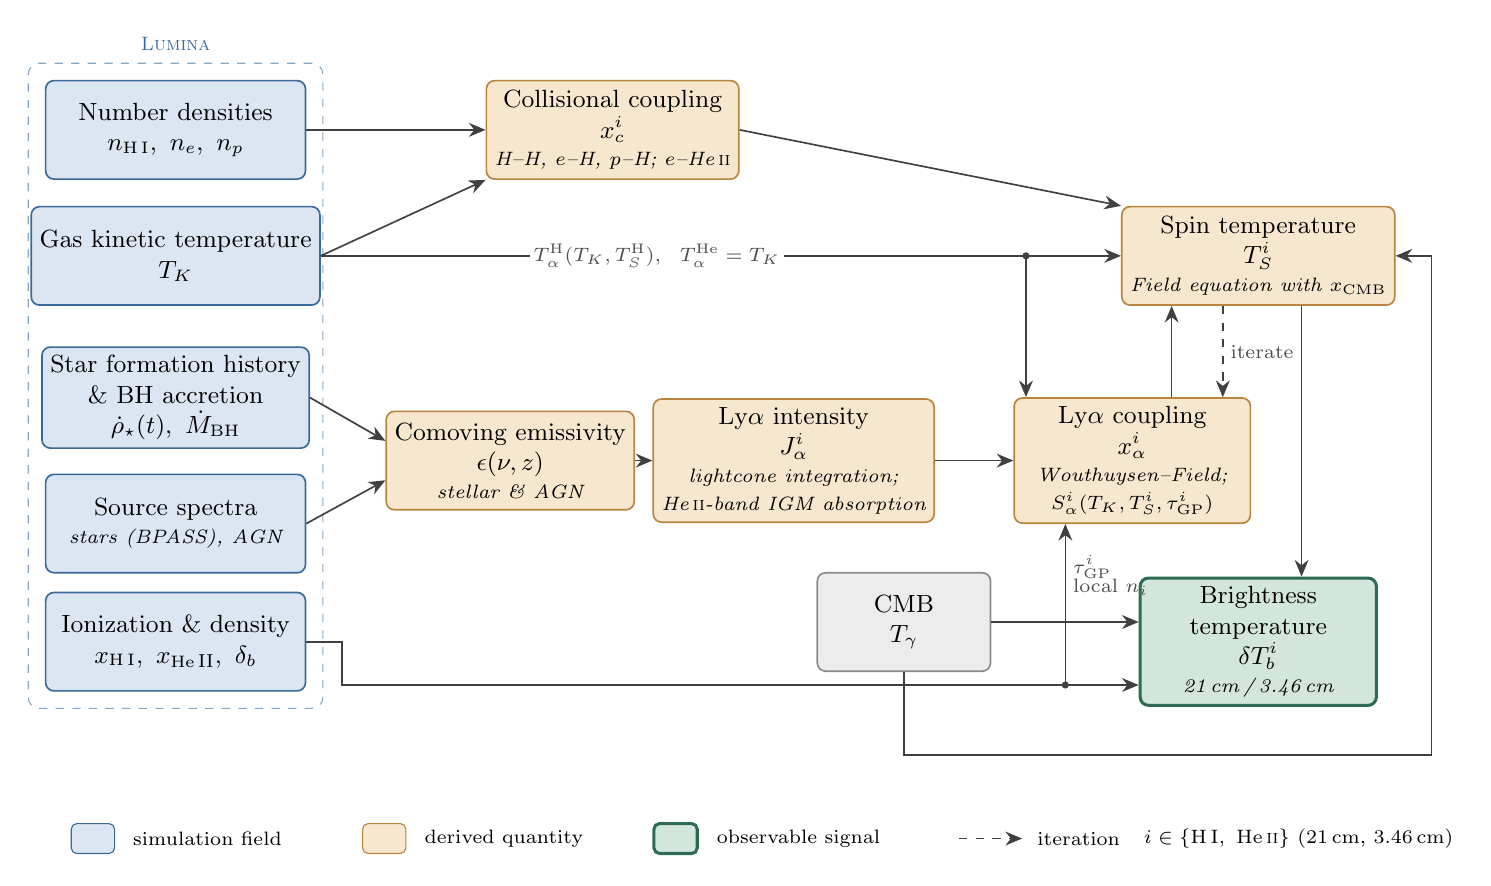
\begin{tikzpicture}[
    font=\small,
    box/.style={rounded corners=3pt, align=center, minimum height=1.25cm, inner sep=3pt, line width=0.6pt},
    sim/.style={box, fill=simfill, draw=simdraw, minimum width=3.3cm},
    der/.style={box, fill=derfill, draw=derdraw, minimum width=3.0cm},
    obs/.style={box, fill=obsfill, draw=obsdraw, line width=1.1pt, minimum width=3.0cm, minimum height=1.5cm},
    cmb/.style={box, fill=cmbfill, draw=cmbdraw, minimum width=2.2cm},
    arr/.style={-{Stealth[length=6pt,width=5pt]}, draw=linecol, line width=0.6pt},
    iter/.style={arr, dashed},
    lab/.style={font=\scriptsize, text=black!70, fill=white, inner sep=1.5pt},
]

% ---------------- simulation fields (left column) ----------------
\node[sim] (dens) at (1.65, 9.0) {Number densities\\ $n_\mathrm{H\,I},\ n_e,\ n_p$};
\node[sim] (TK)   at (1.65, 7.4) {Gas kinetic temperature\\ $T_K$};
\node[sim] (SF)   at (1.65, 5.6) {Star formation history\\ \& BH accretion\\ $\dot\rho_\star(t),\ \dot M_\mathrm{BH}$};
\node[sim] (spec) at (1.65, 4.0) {Source spectra\sub{stars (BPASS), AGN}};
\node[sim] (ion)  at (1.65, 2.5) {Ionization \& density\\ $x_\mathrm{H\,I},\ x_\mathrm{\ionii{He}},\ \delta_b$};
\node[draw=simdraw!60, dashed, rounded corners=4pt, inner sep=6pt, fit=(dens)(ion)] (lum) {};
\node[font=\scriptsize\scshape, text=simdraw, above=1pt of lum.north] {Lumina};

% ---------------- derived quantities ----------------
\node[der] (xc)  at (7.2, 9.0)  {Collisional coupling\\ $x_c^i$\sub{H--H, $e$--H, $p$--H; $e$--\ionii{He}}};
\node[der] (eps) at (5.9, 4.8)  {Comoving emissivity\\ $\epsilon(\nu, z)$\sub{stellar \& AGN}};
\node[der] (J)   at (9.5, 4.8)  {Ly$\alpha$ intensity\\ $J_\alpha^i$\sub{lightcone integration;}\sub{\ionii{He}-band IGM absorption}};
\node[der] (xa)  at (13.8, 4.8) {Ly$\alpha$ coupling\\ $x_\alpha^i$\sub{Wouthuysen--Field;}\sub{$S_\alpha^i(T_K, T_S^i, \tau^i_\mathrm{GP})$}};
\node[der] (TS)  at (15.4, 7.4) {Spin temperature\\ $T_S^i$\sub{Field equation with $x_\mathrm{CMB}$}};

% ---------------- CMB and observable ----------------
\node[cmb] (cmb) at (10.9, 2.75) {CMB\\ $T_\gamma$};
\node[obs] (Tb)  at (15.4, 2.5) {Brightness\\ temperature\\ $\delta T_b^i$\sub{21\,cm\,/\,3.46\,cm}};

% ---------------- arrows ----------------
\draw[arr] (dens.east) -- (xc.west);
\draw[arr] (TK.east) -- (xc.south west);
\draw[arr] (xc.east) -- (TS.north west);

% T_K -> T_S, labelled with the colour temperature; branch down to the Ly-alpha coupling (S_alpha needs T_K)
\draw[arr] (TK.east) -- node[lab, pos=0.42] {$T_\alpha^\mathrm{H}(T_K, T_S^\mathrm{H}),\ \ T_\alpha^\mathrm{He} = T_K$} (TS.west);
\coordinate (br) at (12.45, 7.4);
\fill[linecol] (br) circle (1.3pt);
\draw[arr] (br) -- (12.45, 4.8 |- xa.north);

\draw[arr] (SF.east)   -- ($(eps.west)+(0,0.25)$);
\draw[arr] (spec.east) -- ($(eps.west)+(0,-0.25)$);
\draw[arr] (eps.east) -- (J.west);
\draw[arr] (J.east) -- (xa.west);

% Ly-alpha coupling -> T_S, and the iteration back (T_alpha, S_alpha and x_CMB depend on T_S)
\draw[arr]  (14.3, 0 |- xa.north) -- (14.3, 0 |- TS.south);
\draw[iter] (14.95, 0 |- TS.south) -- node[lab, right=1pt, fill=none] {iterate} (14.95, 0 |- xa.north);

% T_S -> brightness temperature
\draw[arr] (15.95, 0 |- TS.south) -- (15.95, 0 |- Tb.north);

% CMB -> brightness temperature and -> T_S (around the right)
\draw[arr] (cmb.east) -- (cmb.east -| Tb.west);
\draw[arr] (cmb.south) -- ++(0,-1.05) -| (17.6, 7.4) -- (TS.east);

% ionization & density -> brightness temperature, with the branch to tau_GP (local n_HI, n_HeII)
\draw[arr] (ion.east) -- ++(0.45,0) |- ($(Tb.west)+(0,-0.55)$);
\coordinate (br2) at (12.95, 0 |- {$(Tb.west)+(0,-0.55)$});
\fill[linecol] (br2) circle (1.3pt);
\draw[arr] (br2) -- (12.95, 0 |- xa.south) node[lab, pos=0.68, right=1pt, align=left, fill=none] {$\tau^i_\mathrm{GP}$\\[-1pt]local $n_i$};

% ---------------- legend ----------------
\begin{scope}[yshift=-0.2cm]
  \node[fill=simfill, draw=simdraw, rounded corners=2pt, minimum width=0.55cm, minimum height=0.38cm] (l1) at (0.6, 0.2) {};
  \node[right=3pt of l1, font=\scriptsize] {simulation field};
  \node[fill=derfill, draw=derdraw, rounded corners=2pt, minimum width=0.55cm, minimum height=0.38cm] (l2) at (4.3, 0.2) {};
  \node[right=3pt of l2, font=\scriptsize] {derived quantity};
  \node[fill=obsfill, draw=obsdraw, line width=1.1pt, rounded corners=2pt, minimum width=0.55cm, minimum height=0.38cm] (l3) at (8.0, 0.2) {};
  \node[right=3pt of l3, font=\scriptsize] {observable signal};
  \draw[iter] (11.6, 0.2) -- (12.4, 0.2);
  \node[right=2pt, font=\scriptsize] at (12.4, 0.2) {iteration};
  \node[font=\scriptsize, anchor=east] at (18.0, 0.2) {$i \in \{\mathrm{H\,I},\ \mathrm{\ionii{He}}\}$ (21\,cm, 3.46\,cm)};
\end{scope}
\end{tikzpicture}
\end{document}
